\documentclass{article}

\usepackage{blindtext}
\usepackage{multicol}
\usepackage{caption}
\usepackage{amsmath}
\usepackage{tikz}
\usepackage{pgfplots}
\usepackage{hyperref}
\hypersetup{
    colorlinks=true,
    linkcolor=blue,
    filecolor=magenta,
    urlcolor=cyan,
}
\usepackage{geometry}
\geometry{
	a4paper,
	noheadfoot=true,
	left=1.0in,
	right=1.0in,
	top=1.0in,
	bottom=1.0in
}

% url package
\usepackage{hyperref}
\usepackage{subcaption}
\usepackage{relsize} % make some math large
\usepackage{bm} % make some math bold

% Itemize formating
\usepackage{enumitem}

% Figure positioning
\usepackage{float}

% Titling and Author
\title{Latex Tikz Examples, Node-based Diagrams}
\author{\href{https://fanwangecon.github.io/}{Fan Wang}\thanks{\url{https://fanwangecon.github.io}, repository: \href{https://fanwangecon.github.io/Tex4Econ/}{Tex4Econ}}}
\date{\today}

\begin{document}

\maketitle

\section{Connecting Nodes with Arrows}

In the following example, there are three sets of data, relevant for three research objectives:

\begin{verbatim}
    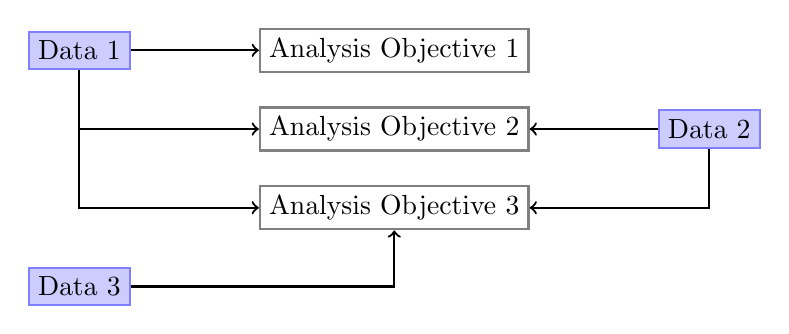
\begin{tikzpicture}[thick]
        \node(1) at (-1,-1) [rectangle,draw=blue!50,fill=blue!20] {Data 1};
        \node(2) at (7 ,-2) [rectangle,draw=blue!50,fill=blue!20] {Data 2};
        \node(3) at (-1,-4) [rectangle,draw=blue!50,fill=blue!20] {Data 3};
        
        \node(4) at (3,-1) [rectangle,draw=black!50] {Analysis Objective 1};
        \node(5) at (3,-2) [rectangle,draw=black!50] {Analysis Objective 2};
        \node(6) at (3,-3) [rectangle,draw=black!50] {Analysis Objective 3};
        
        \draw [->] (1) edge (4);
        \draw [->] (1) |- (5);
        \draw [->] (1) |- (6);
        
        \draw [->] (2) edge (5);
        \draw [->] (2) |- (6);
        
        \draw [->] (3) -| (6);
    \end{tikzpicture}    
\end{verbatim}

\medskip
\begin{center}
    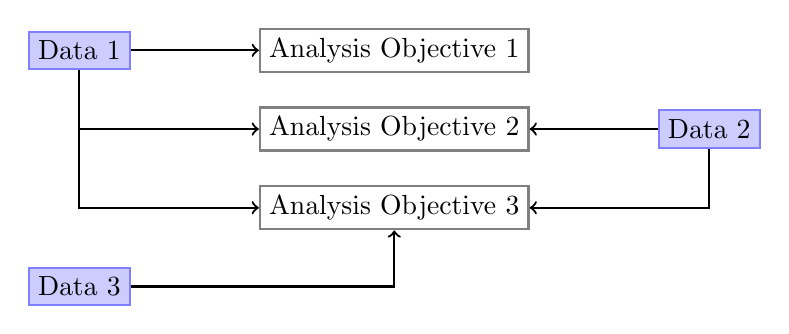
\begin{tikzpicture}[thick]
        \node(1) at (-1,-1) [rectangle,draw=blue!50,fill=blue!20] {Data 1};
        \node(2) at (7 ,-2) [rectangle,draw=blue!50,fill=blue!20] {Data 2};
        \node(3) at (-1,-4) [rectangle,draw=blue!50,fill=blue!20] {Data 3};
        
        \node(4) at (3,-1) [rectangle,draw=black!50] {Analysis Objective 1};
        \node(5) at (3,-2) [rectangle,draw=black!50] {Analysis Objective 2};
        \node(6) at (3,-3) [rectangle,draw=black!50] {Analysis Objective 3};
        
        \draw [->] (1) edge (4);
        \draw [->] (1) |- (5);
        \draw [->] (1) |- (6);
        
        \draw [->] (2) edge (5);
        \draw [->] (2) |- (6);
        
        \draw [->] (3) -| (6);
    \end{tikzpicture}
\end{center}
\clearpage


\section{Connecting Blocks of Nodes and with Blocks of Nodes}

To present the relationship between data and research analysis, show visually how several research aim will be achieved with different data structures and analysis. 

\begin{verbatim}
    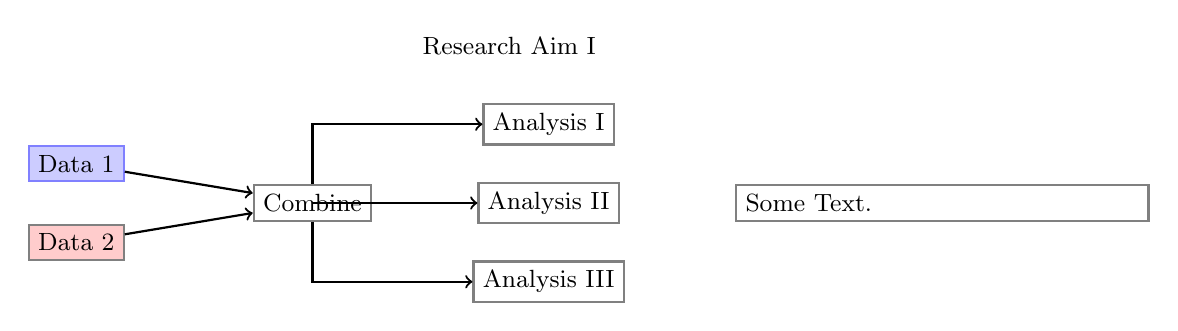
\begin{tikzpicture}[thick, font=\small]
        \node(100) at (2.5,10) [rectangle] {Research Aim I};
        \node(101) at (-3,8.5) [rectangle, draw=blue!50, fill=blue!20] {Data 1};
        \node(102) at (-3,7.5) [rectangle, draw=black!50, fill=red!20] {Data 2};
        \node(111) at (0,8) [rectangle, draw=black!50] {Combine};
        \draw [->] (101) edge (111);
        \draw [->] (102) edge (111);
        \node(121) at (3,9) [rectangle, draw=black!50] {Analysis I};
        \node(122) at (3,8) [rectangle, draw=black!50] {Analysis II};
        \node(123) at (3,7) [rectangle, draw=black!50] {Analysis III};
        \draw [->] (111) |- (121);
        \draw [->] (111) |- (122);
        \draw [->] (111) |- (123);
        \node(131) at (8,8) [rectangle, draw=black!50, text width=5cm] {Some Text.};
    \end{tikzpicture}    
\end{verbatim}

\begin{center}
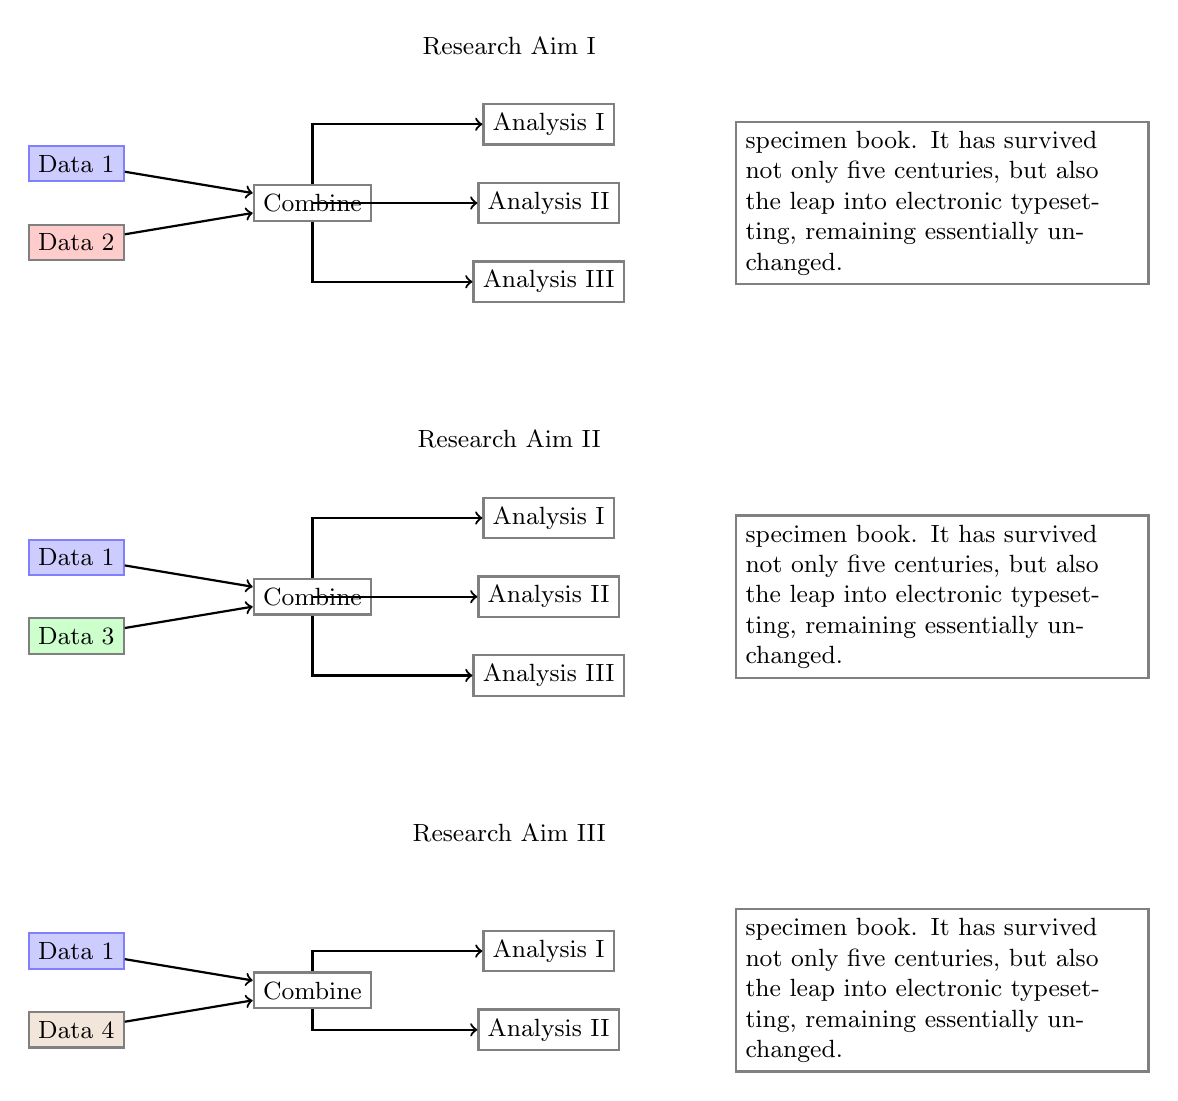
\begin{tikzpicture}[thick, font=\small]
    % Objective I
    \node(100) at (2.5,10) [rectangle] {Research Aim I};
    \node(101) at (-3,8.5) [rectangle, draw=blue!50, fill=blue!20] {Data 1};
    \node(102) at (-3,7.5) [rectangle, draw=black!50, fill=red!20] {Data 2};
    
    \node(111) at (0,8) [rectangle, draw=black!50] {Combine};
    \draw [->] (101) edge (111);
    \draw [->] (102) edge (111);
    
    \node(121) at (3,9) [rectangle, draw=black!50] {Analysis I};
    \node(122) at (3,8) [rectangle, draw=black!50] {Analysis II};
    \node(123) at (3,7) [rectangle, draw=black!50] {Analysis III};
    \draw [->] (111) |- (121);
    \draw [->] (111) |- (122);
    \draw [->] (111) |- (123);
    
    \node(131) at (8,8) [rectangle, draw=black!50, text width=5cm] {specimen book. It has survived not only five centuries, but also the leap into electronic typesetting, remaining essentially unchanged.};
    
    
    % Objective II
    \node(200) at (2.5,5) [rectangle] {Research Aim II};
    \node(201) at (-3,3.5) [rectangle, draw=blue!50, fill=blue!20] {Data 1};
    \node(202) at (-3,2.5) [rectangle, draw=black!50, fill=green!20] {Data 3};
    
    \node(211) at (0,3) [rectangle, draw=black!50] {Combine};
    \draw [->] (201) edge (211);
    \draw [->] (202) edge (211);
    
    \node(221) at (3,4) [rectangle, draw=black!50] {Analysis I};
    \node(222) at (3,3) [rectangle, draw=black!50] {Analysis II};
    \node(223) at (3,2) [rectangle, draw=black!50] {Analysis III};
    \draw [->] (211) |- (221);
    \draw [->] (211) |- (222);
    \draw [->] (211) |- (223);

    \node(231) at (8,3) [rectangle, draw=black!50, text width=5cm] {specimen book. It has survived not only five centuries, but also the leap into electronic typesetting, remaining essentially unchanged.};
    
    % Objective III
    \node(300) at (2.5,0) [rectangle] {Research Aim III};
    \node(301) at (-3,-1.5) [rectangle, draw=blue!50, fill=blue!20] {Data 1};
    \node(302) at (-3,-2.5) [rectangle, draw=black!50, fill=brown!20] {Data 4};
    
    \node(311) at (0,-2) [rectangle, draw=black!50] {Combine};
    \draw [->] (301) edge (311);
    \draw [->] (302) edge (311);
    
    \node(321) at (3,-1.5) [rectangle, draw=black!50] {Analysis I};
    \node(322) at (3,-2.5) [rectangle, draw=black!50] {Analysis II};
    \draw [->] (311) |- (321);
    \draw [->] (311) |- (322);
    
    \node(331) at (8,-2) [rectangle, draw=black!50, text width=5cm] {specimen book. It has survived not only five centuries, but also the leap into electronic typesetting, remaining essentially unchanged.};
    
\end{tikzpicture}
\end{center}
\clearpage
\newpage



\section{Rows of Data and Analysis Connected Nodes}

\subsection{Research Plan Diagram Example One}

To present the relationship between data and research analysis, show visually how several research aim will be achieved with different data structures and analysis. 

\begin{figure}[H]
\centering
\caption{Research Aim I---Inequality in Ambient Environmental Exposures}
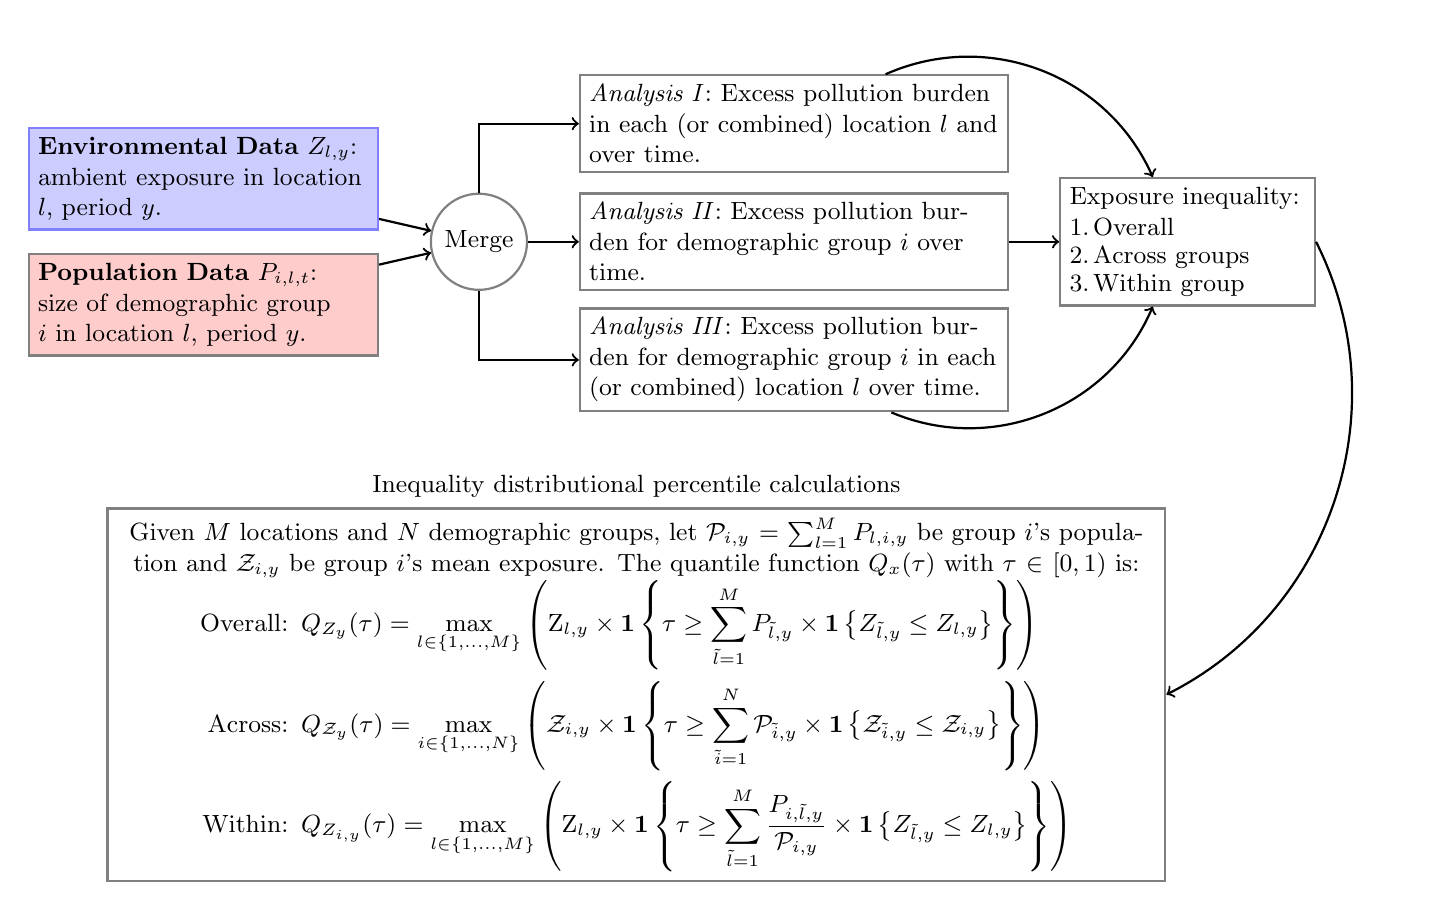
\begin{tikzpicture}[thick, font=\small]
% A. Sizing for tikz
\def\fstdata{4.2cm}
\def\fstanalysis{5.2cm}
\def\fstunequal{3.0cm}
\def\fstnote{13.2cm}
% B.1 Text for tikz group 1
\newcommand{\dataone}{\textbf{Environmental Data} $Z_{l,y}$: ambient exposure in location $l$, period $y$.}
\newcommand{\datatwo}{\textbf{Population Data} $P_{i,l,t}$: size of demographic group $i$ in location $l$, period $y$.}
% B.2 Text for tikz group 2
\newcommand{\analysisone}{\emph{Analysis I}: Excess pollution burden in each (or combined) location $l$ and over time.}
\newcommand{\analysistwo}{\emph{Analysis II}: Excess pollution burden for demographic group $i$ over time.}
\newcommand{\analysisthree}{\emph{Analysis III}: Excess pollution burden for demographic group $i$ in each (or combined) location $l$ over time.}
% B.3 Text for tikz group 3
\newcommand{\inequalitymeasure}{Exposure inequality: 
\begin{enumerate}[leftmargin=0cm,itemindent=.3cm,labelwidth=\itemindent,labelsep=0.0cm, itemsep=-0.1cm, topsep=0cm, align=left]
    \item Overall
    \item Across groups
    \item Within group
\end{enumerate}}
% C Tikz Draw
    % Objective I
    % \node(100) at (2.5,10.75) [rectangle] {};
    \node(101) at (-3,8.8) [rectangle, draw=blue!50, fill=blue!20, text width=\fstdata] {\dataone};
    \node(102) at (-3,7.2) [rectangle, draw=black!50, fill=red!20, text width=\fstdata] {\datatwo};
    
    \node(111) at (0.5,8) [circle, draw=black!50] {Merge};
    \draw [->] (101) edge (111);
    \draw [->] (102) edge (111);
    
    \node(121) at (4.5,9.5) [rectangle, draw=black!50, text width=\fstanalysis] {\analysisone};
    \node(122) at (4.5,8) [rectangle, draw=black!50, text width=\fstanalysis] {\analysistwo};
    \node(123) at (4.5,6.5) [rectangle, draw=black!50, text width=\fstanalysis] {\analysisthree};
    \draw [->] (111.north) |- (121);
    \draw [->] (111.east) |- (122);
    \draw [->] (111.south) |- (123);
    
    \node(131) at (9.5,8) [rectangle, draw=black!50, text width=\fstunequal] {\inequalitymeasure};
    \draw [->] (121) to [bend left=45] (131);
    \draw [->] (122) to (131);
    \draw [->] (123) to [bend right=45] (131);    
    
    \node(141) at (2.5,2.25) [rectangle, draw=black!50, text width=\fstnote, label={Inequality distributional percentile calculations}, align=center] {
Given $M$ locations and $N$ demographic groups, let $\mathcal{P}_{i,y}=\sum_{l=1}^{M}
P_{l,i,y}$ be group $i$'s population and $\mathcal{Z}_{i,y}$ be group $i$'s mean exposure. The quantile function $Q_{x}(\tau)$ with $\tau\in[0,1)$ is:\\
$\begin{aligned}   
\text{Overall: } &Q_{Z_{y}}(\tau) =
\max_{l\in\left\{1, \dots, M \right\}}
\left(
    \text{Z}_{l,y}
    \times
    \mathbf{1}\left\{
    \tau \ge
      \sum_{\tilde{l}=1}^{M} P_{\tilde{l},y}
      \times
      \mathbf{1}\left\{
        Z_{\tilde{l},y} \le Z_{l,y}
        \right\}
    \right\}
\right)\\
\text{Across: } &Q_{\mathcal{Z}_{y}}(\tau) =
\max_{i\in\left\{1, \dots, N \right\}}
\left(
    \mathcal{Z}_{i,y}
    \times
    \mathbf{1}\left\{
    \tau \ge
      \sum_{\tilde{i}=1}^{N} \mathcal{P}_{\tilde{i},y}
      \times
      \mathbf{1}\left\{
        \mathcal{Z}_{\tilde{i},y} \le \mathcal{Z}_{i,y}
        \right\}
    \right\}
\right)\\
\text{Within: } &Q_{Z_{i,y}}(\tau) =
\max_{l\in\left\{1, \dots, M \right\}}
\left(
    \text{Z}_{l,y}
    \times
    \mathbf{1}\left\{
    \tau \ge
      \sum_{\tilde{l}=1}^{M}
      \frac{P_{i, \tilde{l}, y}}{\mathcal{P}_{i,y}}
      \times
      \mathbf{1}\left\{
        Z_{\tilde{l},y} \le Z_{l,y}
        \right\}
    \right\}
\right)
% , \forall i\in\left\{1,\dots,N\right\}
\end{aligned}$    
    };
\draw [->] (131.east) to [bend left=45] (141.east); 

\end{tikzpicture}
\end{figure}
\clearpage


\subsection{Research Plan Diagram Example Two}

\begin{figure}[H]
\centering
\caption{Research Aim II---Inequality in Ambient Environmental Exposures}
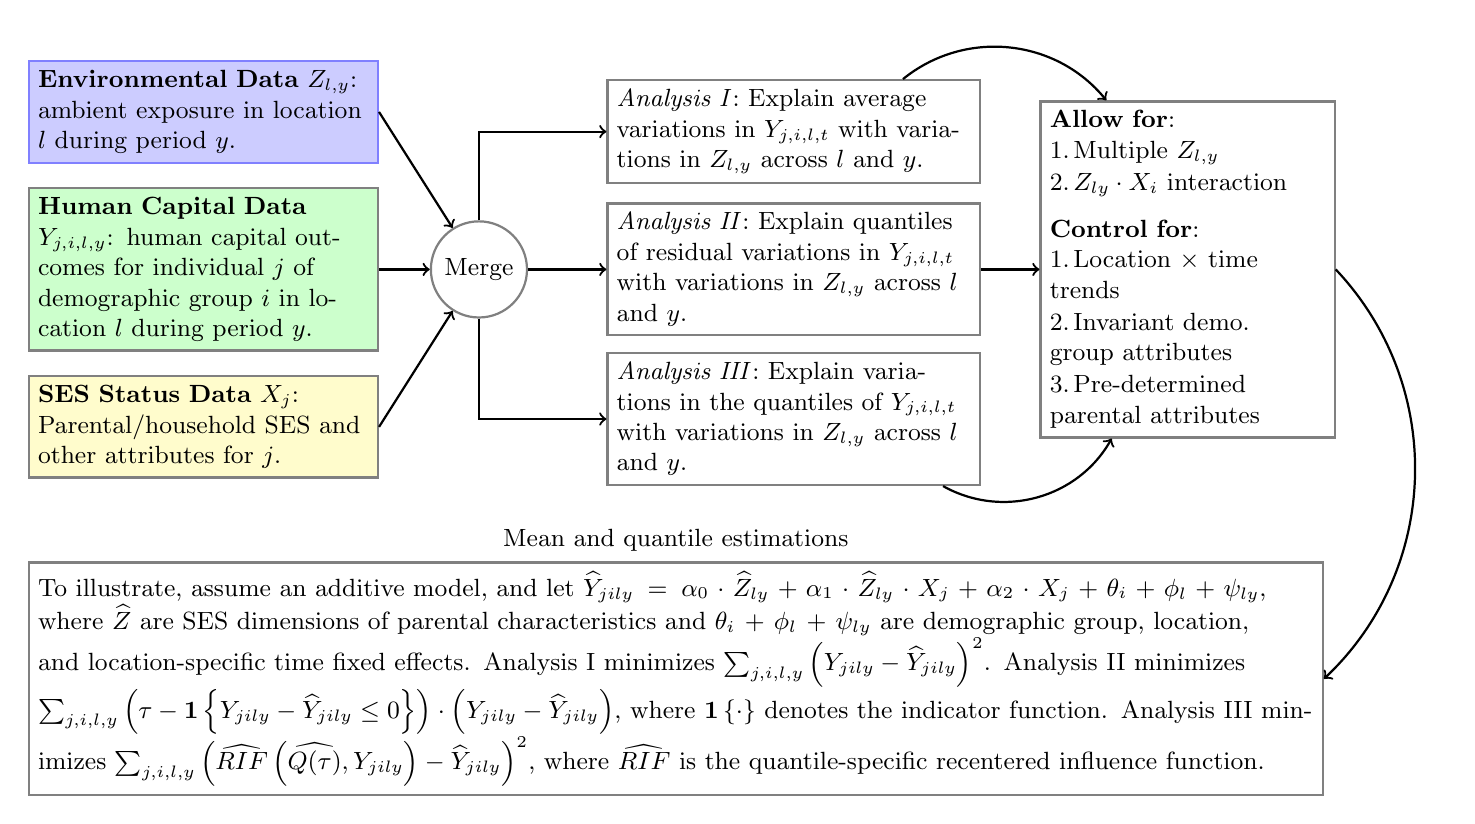
\begin{tikzpicture}[thick, font=\small]
% A. Sizing for tikz
\def\fstdata{4.2cm}
\def\fstanalysis{4.5cm}
\def\fstunequal{3.5cm}
\def\fstnote{16.2cm}
% B.1 Text for tikz group 1
\newcommand{\dataone}{\textbf{Environmental Data} $Z_{l,y}$: ambient exposure in location $l$ during period $y$.}
\newcommand{\datatwo}{\textbf{Human Capital Data} $Y_{j,i,l,y}$: human capital outcomes for individual $j$ of demographic group $i$ in location $l$ during period $y$.}
\newcommand{\datathree}{\textbf{SES Status Data} $X_{j}$: Parental/household SES and other attributes for $j$.}
% B.2 Text for tikz group 2
\newcommand{\analysisone}{\emph{Analysis I}: Explain average variations in $Y_{j,i,l,t}$ with variations in $Z_{l,y}$ across $l$ and $y$.}
\newcommand{\analysistwo}{\emph{Analysis II}: Explain quantiles of residual variations in $Y_{j,i,l,t}$ with variations in $Z_{l,y}$ across $l$ and $y$.}
\newcommand{\analysisthree}{\emph{Analysis III}: Explain variations in the quantiles of $Y_{j,i,l,t}$ with variations in $Z_{l,y}$ across $l$ and $y$.}
% B.3 Text for tikz group 3
\newcommand{\inequalitymeasure}{
\textbf{Allow for}: 
\begin{enumerate}[leftmargin=0cm,itemindent=.3cm,labelwidth=\itemindent,labelsep=0cm, itemsep=-0.05cm, topsep=0cm, align=left]
    \item Multiple $Z_{l,y}$ 
    \item $Z_{ly} \cdot X_{i}$ interaction
    % \item Instruments (e.g. thermal inversion)
\end{enumerate}
\medskip
\textbf{Control for}: 
\begin{enumerate}[leftmargin=0cm,itemindent=.3cm,labelwidth=\itemindent,labelsep=0cm, itemsep=-0.05cm, topsep=0cm, align=left]
    \item Location $\times$ time trends
    \item Invariant demo. group attributes
    \item Pre-determined parental attributes
\end{enumerate}}
% C Tikz Draw
    % Objective I
    % \node(100) at (2.5,10.75) [rectangle] {};
    \node(101) at (-3,10) [rectangle, draw=blue!50, fill=blue!20, text width=\fstdata] {\dataone};
    \node(102) at (-3,8) [rectangle, draw=black!50, fill=green!20, text width=\fstdata] {\datatwo};
    \node(103) at (-3,6) [rectangle, draw=black!50, fill=yellow!20, text width=\fstdata] {\datathree};
    
    
    \node(111) at (0.5,8) [circle, draw=black!50] {Merge};
    \draw [->] (101.east) to (111);
    \draw [->] (102) edge (111);
    \draw [->] (103.east) to (111);
    
    \node(121) at (4.5,9.75) [rectangle, draw=black!50, text width=\fstanalysis] {\analysisone};
    \node(122) at (4.5,8) [rectangle, draw=black!50, text width=\fstanalysis] {\analysistwo};
    \node(123) at (4.5,6.1) [rectangle, draw=black!50, text width=\fstanalysis] {\analysisthree};
    \draw [->] (111.north) |- (121);
    \draw [->] (111.east) |- (122);
    \draw [->] (111.south) |- (123);
    
    \node(131) at (9.5,8) [rectangle, draw=black!50, text width=\fstunequal] {\inequalitymeasure};
    \draw [->] (121) to [bend left=45] (131);
    \draw [->] (122) to (131);
    \draw [->] (123) to [bend right=45] (131);    
    
    \node(141) at (3.00,2.8) [rectangle, draw=black!50, text width=\fstnote, label={Mean and quantile estimations}, align=left] {To illustrate, assume an additive model, and let $\widehat{Y}_{jily}= 
\alpha_0 \cdot \widehat{Z}_{ly}
+ \alpha_1 \cdot \widehat{Z}_{ly} \cdot X_{j}
+ \alpha_2 \cdot X_{j}
+ \theta_{i}
+ \phi_{l}
+ \psi_{ly}$, 
where $\widehat{Z}$ are SES dimensions of parental characteristics and $\theta_{i}
+ \phi_{l}
+ \psi_{ly}$ are demographic group, location, and location-specific time fixed effects.
Analysis I minimizes 
$\sum_{j,i,l,y} \left(Y_{jily} - \widehat{Y}_{jily}\right)^2$. 
Analysis II minimizes 
$\sum_{j,i,l,y} 
\left(\tau-
\mathbf{1}
\left\{ Y_{jily} - \widehat{Y}_{jily} \le 0\right\}
\right) \cdot \left(Y_{jily} - \widehat{Y}_{jily}\right)
$, where $\mathbf{1}\left\{\cdot\right\}$ denotes the indicator function.
Analysis III minimizes 
$\sum_{j,i,l,y} 
\left(\widehat{RIF}\left(\widehat{Q(\tau)}, Y_{jily}\right) - 
\widehat{Y}_{jily}\right)^2$, where $\widehat{RIF}$ is the quantile-specific recentered influence function.
};
\draw [->] (131.east) to [bend left=45] (141.east); 

\end{tikzpicture}
\end{figure}

\clearpage

\subsection{Research Plan Diagram Example Three}

\begin{figure}[H]
\centering
\caption{Research Aim III---Inequality in Ambient Environmental Exposures}
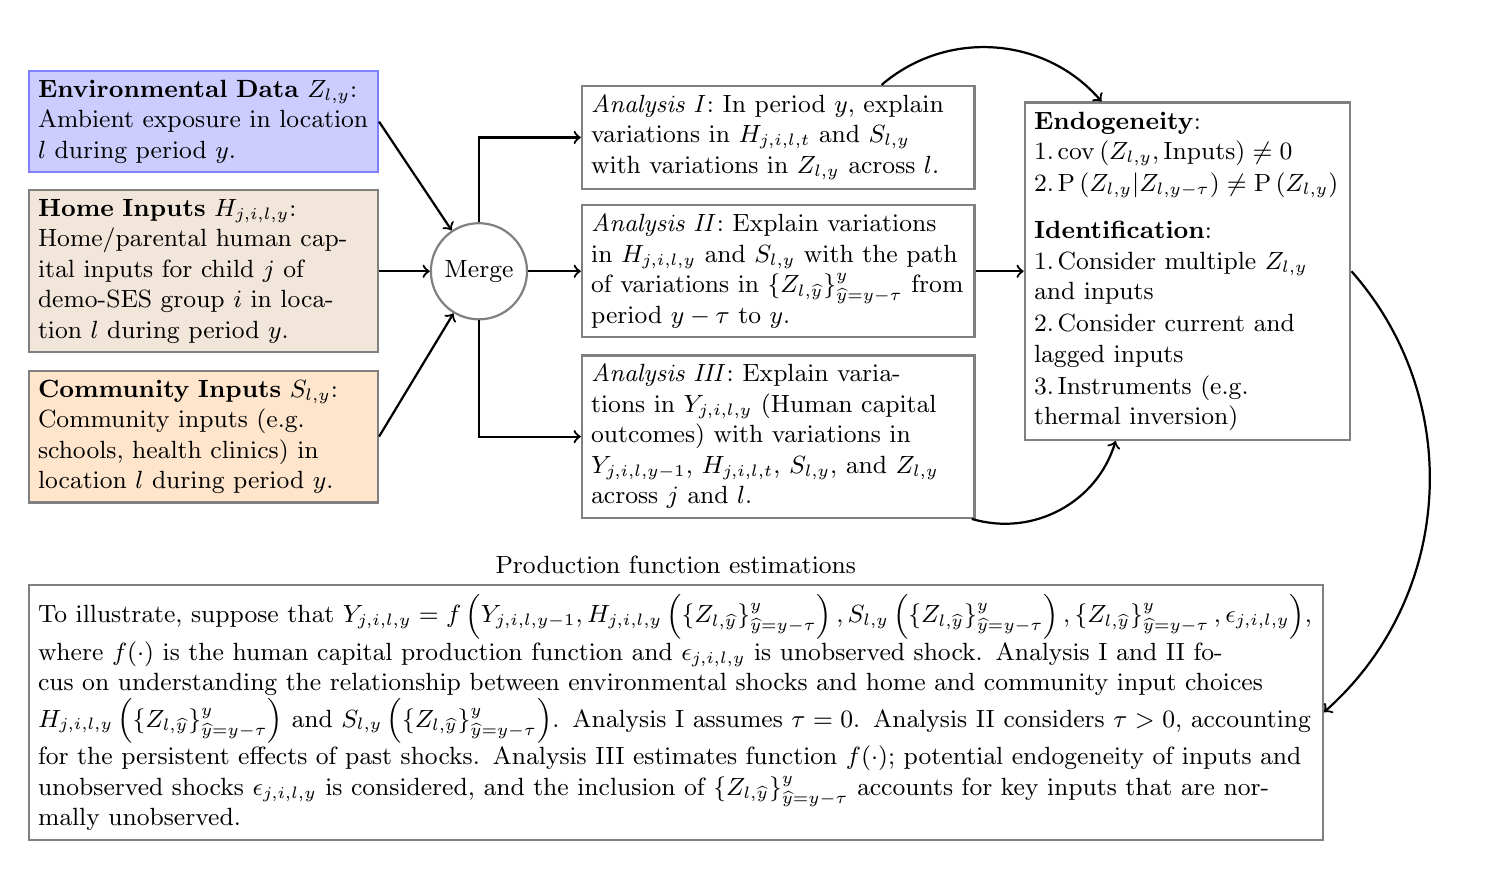
\begin{tikzpicture}[thick, font=\small]
% A. Sizing for tikz
\def\fstdata{4.2cm}
\def\fstanalysis{4.75cm}
\def\fstunequal{3.90cm}
\def\fstnote{16.2cm}
% B.1 Text for tikz group 1
\newcommand{\dataone}{\textbf{Environmental Data} $Z_{l,y}$: Ambient exposure in location $l$ during period $y$.}
\newcommand{\datatwo}{\textbf{Home Inputs} $H_{j,i,l,y}$: Home/parental human capital inputs for child $j$ of demo-SES group $i$ in location $l$ during period $y$.}
\newcommand{\datathree}{\textbf{Community Inputs} $S_{l,y}$: Community inputs (e.g. schools, health clinics) in location $l$ during period $y$.}
% B.2 Text for tikz group 2
\newcommand{\analysisone}{\emph{Analysis I}: In period $y$, explain variations in $H_{j,i,l,t}$ and $S_{l,y}$ with variations in $Z_{l,y}$ across $l$.}
\newcommand{\analysistwo}{\emph{Analysis II}:
Explain variations in $H_{j,i,l,y}$ and $S_{l,y}$ with the path of variations in $\left\{Z_{l,\widehat{y}}\right\}_{\widehat{y}=y-\tau}^{y}$ from period $y-\tau$ to $y$.
% Evaluate the persistence of the association between $Y_{j,i,l,y}$ and $Z_{l,y-\tau}$ from $\tau$ periods ago, considering $Z_{l,y}$.
}
\newcommand{\analysisthree}{\emph{Analysis III}: Explain variations in $Y_{j,i,l,y}$ (Human capital outcomes) with variations in $Y_{j,i,l,y-1}$, $H_{j,i,l,t}$, $S_{l,y}$, and $Z_{l,y}$ across $j$ and $l$.}
% B.3 Text for tikz group 3
\newcommand{\inequalitymeasure}{
\textbf{Endogeneity}: 
\begin{enumerate}[leftmargin=0cm,itemindent=.3cm,labelwidth=\itemindent,labelsep=0cm, itemsep=-0.05cm, topsep=0cm, align=left]
    % \item Multiple $Z_{l,y}$ 
    % \item $Z_{ly} \cdot X_{i}$ interaction
    % \item Isolate unpredictable components of $Z_{l,y}$ 
    \item $\mathrm{cov}\left(Z_{l,y},\text{Inputs}\right)\neq 0$ 
    \item $\mathrm{P}\left(Z_{l,y}|Z_{l,y-\tau}\right)\neq \mathrm{P}\left(Z_{l,y}\right)$
    % \item Instruments (e.g. thermal inversion)
\end{enumerate}
\medskip
\textbf{Identification}: 
\begin{enumerate}[leftmargin=0cm,itemindent=.3cm,labelwidth=\itemindent,labelsep=0cm, itemsep=-0.05cm, topsep=0cm, align=left]
    \item Consider multiple $Z_{l,y}$ and inputs
    \item Consider current and lagged inputs
    \item Instruments (e.g. thermal inversion)
\end{enumerate}}
% C Tikz Draw
    % Objective I
    % \node(100) at (2.5,10.75) [rectangle] {};
    \node(101) at (-3,9.9) [rectangle, draw=blue!50, fill=blue!20, text width=\fstdata] {\dataone};
    \node(102) at (-3,8.0) [rectangle, draw=black!50, fill=brown!20, text width=\fstdata] {\datatwo};
    \node(103) at (-3,5.9) [rectangle, draw=black!50, fill=orange!20, text width=\fstdata] {\datathree};
    
    
    \node(111) at (0.5,8) [circle, draw=black!50] {Merge};
    \draw [->] (101.east) to (111);
    \draw [->] (102) edge (111);
    \draw [->] (103.east) to (111);
    
    \node(121) at (4.3,9.7) [rectangle, draw=black!50, text width=\fstanalysis] {\analysisone};
    \node(122) at (4.3,8.0) [rectangle, draw=black!50, text width=\fstanalysis] {\analysistwo};
    \node(123) at (4.3,5.9) [rectangle, draw=black!50, text width=\fstanalysis] {\analysisthree};
    \draw [->] (111.north) |- (121);
    \draw [->] (111.east) to (122);
    \draw [->] (111.south) |- (123);
    
    \node(131) at (9.5,8) [rectangle, draw=black!50, text width=\fstunequal] {\inequalitymeasure};
    \draw [->] (121) to [bend left=45] (131);
    \draw [->] (122) to (131);
    \draw [->] (123) to [bend right=45] (131);    
    
    \node(141) at (3.00,2.4) [rectangle, draw=black!50, text width=\fstnote, label={Production function estimations}, align=left] {To illustrate, suppose that $Y_{j,i,l,y}=f\left(
    Y_{j,i,l,y-1},
    H_{j,i,l,y}\left(\left\{Z_{l,\widehat{y}}\right\}_{\widehat{y}=y-\tau}^{y}\right),
    S_{l,y}\left(\left\{Z_{l,\widehat{y}}\right\}_{\widehat{y}=y-\tau}^{y}\right),
    \left\{Z_{l,\widehat{y}}\right\}_{\widehat{y}=y-\tau}^{y},
    \epsilon_{j,i,l,y}
    \right)$, where $f(\cdot)$ is the human capital production function and $\epsilon_{j,i,l,y}$ is unobserved shock. Analysis I and II focus on understanding the relationship between environmental shocks and home and community input choices $H_{j,i,l,y}\left(\left\{Z_{l,\widehat{y}}\right\}_{\widehat{y}=y-\tau}^{y}\right)$ and $S_{l,y}\left(\left\{Z_{l,\widehat{y}}\right\}_{\widehat{y}=y-\tau}^{y}\right)$. Analysis I assumes $\tau =0$. Analysis II considers $\tau >0$, accounting for the persistent effects of past shocks. Analysis III estimates function $f(\cdot)$; potential endogeneity of inputs and unobserved shocks $\epsilon_{j,i,l,y}$ is considered, and the inclusion of $\left\{Z_{l,\widehat{y}}\right\}_{\widehat{y}=y-\tau}^{y}$ accounts for key inputs that are normally unobserved.
};
\draw [->] (131.east) to [bend left=45] (141.east); 

\end{tikzpicture}
\end{figure}



\clearpage
\section{Multi-stage Choice Diagram}

Three nodes, two in a row.

\tikzset{
    % Two node styles for game trees: solid and hollow
    solid node/.style={circle,draw,inner sep=1.5,fill=black},
    hollow node/.style={circle,draw,inner sep=1.5,fill=white}
}
\begin{center}
\begin{tikzpicture}[scale=1.5,font=\footnotesize]

% A.2 Level Styles
    % Specify spacing for each level of the tree
    \tikzstyle{level 1}=[level distance=17mm,sibling distance=25mm]
    \tikzstyle{level 2}=[level distance=15mm,sibling distance=15mm]

% B Level 1 point
\node(0)[solid node,label=above:{$P1$}]{}

% C Level 2 Node (child nodes)
% C.1 First child node, left
child{
    % C.1.a Node line color
    [red]
    % C.1.b Node dot
    node(1)[solid node, label=below:{red dot}]{}
    % C.1.c now go to edge
    edge from parent
        % C.1.c Node along edge
        node[sloped, above, black, text width=3cm]{Minimum Choice showing up along this red line}
    }
% C.2 Middle Child node, do not show line, invisible
child{
    % Main node of level 2 middle node, same y-axis height as node left and right
    % Y-shift to move level 3 child node lower
    [red]  % this is the style of the line middle line
        node(2)[solid node, xshift=30, yshift=-50, label=right:{hello}]{} % this is the style of the middle point that would have matched up the middle line
    % D.1 Left level 3 (from middle level 2)
    child{
        [black]
        node[hollow node,label=below:{$(a,b)$}]{}
        edge from parent
            node[left]{$C$}
        }
    child{
        [black]
        node[hollow node,label=below:{$(c,d)$}]{}
        edge from parent
            node[right]{$D$}
        }
    edge from parent
        % draw none here prevents the middle line extending rom P1 to hello to be drawn
        [draw=none]
        %note that you need to adjust the yshift if you change the level distance
        node[left, black, xshift=-5, yshift=0, text width = 1mm]{$\alpha$\\$\beta$\\$\sigma$}
    }
child{
    [black]
    node(3)[solid node, label=right:{hi there}, green]{}
    edge from parent
        node[right, xshift=0, yshift=15, text width=2cm]{Some text for this edge}
    };
% information set
\draw[dashed, bend right]
    (1) to (3);
\draw[dashed, bend left, line width=0.5mm, blue]
    (0) to
        node[right, text width=1.25cm, xshift=5, yshift=-10]
            {\tiny{label right of blue dashed line}}
        (2);
\end{tikzpicture}
\end{center}

\end{document}
